\subsection{Distribuição das Flutuações}\label{sec:5.3}
O desvio de energia $\epsilon$ em qualquer instante $t$ é o resultado da superposição das contribuições das emissões quânticas em todos os tempos anteriores $t_i$. Então pode-se escrever que
\begin{align}
	\epsilon(t) = \sum\limits_{t_i<t}^{}u_i e^{-(t-t_i)\alpha_\epsilon}cos(\Omega(t-t_i))\label{eq:5.49}
\end{align}
onde $u_i$ é a energia quântica emitida no tempo $t_i$. Como o valor típico de $\epsilon(t)$ é muito maior que a energia quântica típica -- veja a equação \eqref{eq:5.32} -- e os tempos $t_i$ são aleatoriamente distribuídos, a soma em qualquer instante $t$ consiste de contribuições de vários termos pequenos, os quais são estatisticamente independentes, e que tem probabilidades iguais de serem positivos ou negativos. É sabido\footnote{E vem do Teorema Central do Limite da teoria de probabilidade.} que o resultado desta soma é uma quantidade estocástica cujo valor provável é zero e sua variância segue uma distribuição normal -- uma distribuição conhecida como Gaussiana. Isto é, a probabilidade $w(\epsilon)d\epsilon$ do desvio de energia estar dentro do intervalo $d\epsilon$ em $\epsilon$ é distribuída de acordo com
\begin{align}
	w(\epsilon)d\epsilon = \frac{1}{\sqrt{2\pi}\sigma_\epsilon}\ e^{-\epsilon^2/2\sigma_\epsilon^2}d\epsilon\label{eq:5.50}
\end{align}
O parâmetro $\sigma_\epsilon$ é chamado de desvio padrão e é igual ao valor RMS do espalhamento da distribuição -- isto é, a raiz quadrada de $\mean{\epsilon^2}$ -- e pode ser facilmente demonstrado pela integração direta:
\begin{align}
	\sigma_\epsilon^2 = \int\limits_{-\infty}^{+\infty}\epsilon^2w(\epsilon)d\epsilon
\end{align}
(A função da distribuição $w(\epsilon)$ é normalizada de forma apropriada para que sua integral completa seja igual a 1.) O desvio padrão $\sigma_\epsilon$ é, portanto, a mesma quantidade que foi avaliada anteriormente.

Em um feixe de elétrons existe, normalmente, um número $N$ grande de elétrons armazenados. Enquanto as interações entre os elétrons puderem ser ignoradas, a distribuição de energias em um \textit{bunch} irá -- em condições estacionárias -- também ser descrita pela equação \eqref{eq:5.50}. Desta forma, o número de elétrons com energias entre $\epsilon$ e $\epsilon + d\epsilon$ será apenas $Nw(\epsilon)d\epsilon$. E a "largura média" do \textit{spread} de energia do feixe será descrita por $\sigma_\epsilon$.

Tanto a função de distribuição da equação \eqref{eq:5.50} quanto o cálculo de $\sigma_\epsilon$ assumem que as oscilações de energia são lineares (considerando as não-linearidades, a equação \eqref{eq:5.49} não é correta e os efeitos de uma emissão quântica individual não são mais independentes). No entanto, já foi visto que as oscilações de energia não são lineares para grandes desvios de energia. Se a função da tensão de RF é significantemente não-linear nos desvios de tempo correspondentes aos desvios de energia em questão, deve-se esperar que a distribuição de probabilidade para $\epsilon$ seja distorcida com relação a distribuição ideal da equação \eqref{eq:5.50}. Porém, caso a não-linearidade não seja muito grande na maior parte da distribuição, espera-se que tanto $\sigma_\epsilon$ quanto a função de distribuição dos desvios de energia não sejam muito afetados.

A distribuição dos \textit{spreads} de energia considerada implica em distribuições relacionadas a outros parâmetros das oscilações de energia. As relações entre elas são mais facilmente entendidas considerando a trajetória do elétron em um diagrama de espaço de fase, do mesmo tipo que foi discutido na \autoref{sec:3.5}. Suponha que o estado de uma oscilação de energia seja dado pelo seu desvio de energia $\epsilon$ e seu desvio de tempo "dimensionado" $\theta$ definido por
\begin{align}
	\theta = \frac{\Omega E_0}{\alpha}\tau\label{eq:5.52}
\end{align}
onde $\Omega$ é a frequência angular da oscilação de energia e $\alpha$ é o fator de compactação de momento, ambos constantes. Desta forma, $\theta$ difere por apenas um fator de escala de $\tau$, o desvio de tempo original das oscilações de energia (veja a \autoref{sec:3.5}). Enquanto a taxa de amortecimento for pequena, $\theta$ pode ser definido de forma equivalente por
\begin{align}
	\theta = \frac{1}{\Omega}\frac{d\epsilon}{dt}
\end{align}
então $\theta$ também pode ser visto como uma derivada normalizada de $\epsilon$.

\begin{proof}
	Na \autoref{sec:3.5} foi visto que $\tau$ e $\epsilon$ podem ser representados utilizando notação complexa:
	\begin{align*}
		\tau(t) = \tilde{\tau}\ e^{-(\alpha_\epsilon - i\Omega)t}\\
		\epsilon(t) = \tilde{\epsilon}\ e^{-(\alpha_\epsilon - i\Omega)t}
	\end{align*}
	onde, se a taxa de amortecimento for pequena ($\alpha_\epsilon << \Omega$), tem-se que as amplitudes de oscilação de cada grandeza estão relacionadas da seguinte maneira:
	\begin{align*}
		\tilde{\epsilon} = -i\frac{\Omega E_0}{\alpha}\tilde{\tau}
	\end{align*}
	Substituindo esta relação na equação de $\epsilon(t)$, tem-se que
	\begin{align*}
		\epsilon(t) &= -i\frac{\Omega E_0}{\alpha}\tilde{\tau}\ e^{-(\alpha_\epsilon - i\Omega)t}\\
					&= -i\frac{\Omega E_0}{\alpha}\tau
	\end{align*}
	Derivando $\epsilon(t)$ com relação ao tempo, tem-se
	\begin{align*}
		\frac{d\epsilon}{dt} = i\frac{\Omega E_0}{\alpha} (\alpha_\epsilon-i\Omega)\tau
	\end{align*}
	Mas já assumiu-se que $\alpha_\epsilon << \Omega$. Então, desprezando $\alpha_\epsilon$, tem-se
	\begin{align*}
		\frac{d\epsilon}{dt} = -i^2\frac{\Omega^2 E_0}{\alpha}\tau = \frac{\Omega^2 E_0}{\alpha}\tau
	\end{align*}
	Substituindo este resultado na equação \eqref{eq:5.52}:
	\begin{align*}
		\theta = \frac{\Omega E_0}{\alpha}\tau = \frac{1}{\Omega}\frac{\Omega^2 E_0}{\alpha}\tau = \frac{1}{\Omega}\frac{d\epsilon}{dt}
	\end{align*}
	c.q.d.
\end{proof}

Agora pode-se representar o estado do movimento de um elétron por um ponto em um gráfico bidimensional onde $\epsilon$ e $\theta$ são coordenadas ortogonais -- veja a \autoref{fig:fig44}(a) -- e onde uma oscilação de amplitude constante é descrita por um círculo. Então, enquanto os efeitos do amortecimento e da emissão quântica forem pequenos, pode-se que considerar que, para qualquer pequeno intervalo de tempo, $\epsilon$ e $\theta$ variam como
\begin{align}
	\epsilon = A\ cos(\varphi)\\
	\theta = A\ sen(\varphi)
\end{align}
onde
\begin{align}
	\varphi = \Omega t - \varphi_0
\end{align}
e $A$ é uma amplitude com variação lenta. Os termos $A$ e $\varphi$ são uma representação na forma polar do ponto em questão, e $\varphi$ aumenta como $\Omega t$.

\begin{figure}[!htb]
	\centering
	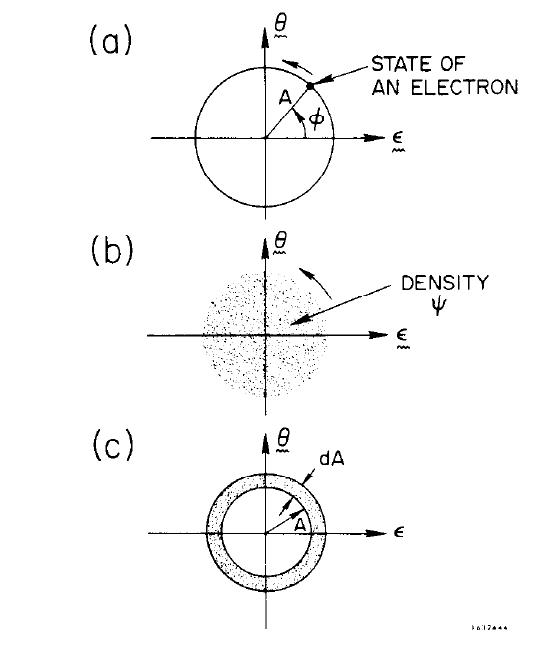
\includegraphics[width=0.6\linewidth]{./Figuras/fig44.jpeg}
	\caption{Espaço de fase dimensionado das oscilações de energia. Retirado de \cite{sands1970physics}.}
	\label{fig:fig44}
\end{figure}

Agora, a distribuição das oscilações de energia dos elétrons em um \textit{bunch} pode ser representada pela distribuição de pontos no diagrama de espaço de fase indicada na esquematicamente na \autoref{fig:fig44}(b). Uma descrição completa da distribuição é dada especificando a densidade $\psi(\epsilon,\theta)$ no plano $\epsilon$,$\theta$. Isto é, $\psi(\epsilon,\theta)d\epsilon d\theta$ representa o número de elétrons encontrados no elemento de área $d\epsilon d\theta$ localizado em $(\epsilon,\theta)$. A projeção de $\psi(\epsilon,\theta)$ no plano horizontal já é conhecida. Se existem $N$ elétrons em um \textit{bunch}, é apenas $Nw(\epsilon)$. Mas em um quarto da oscilação cada elétron rotaciona um quarto de revolução em torno da origem da figura. Já que uma distribuição estacionária está sendo considerada -- isto é, ela não varia com o tempo -- as projeções nos eixos horizontal e vertical devem ser idênticas. Dito isso, o número de elétrons em um elemento de área $d\epsilon d\theta$ deve ser dado por
\begin{align}
	\psi(\epsilon,\theta)d\epsilon d\theta = \frac{N}{2\pi \sigma_\epsilon^2}\ e^{-(\epsilon^2+\theta^2)/2\sigma_\epsilon^2}d\epsilon d\theta\label{eq:5.57}
\end{align}
A projeção no eixo horizontal é
\begin{align*}
	\int \psi(\epsilon,\theta)d\theta = \frac{N}{\sqrt{2\pi}\sigma_\epsilon}\ e^{-\epsilon^2/2\sigma_\epsilon^2}d\epsilon
\end{align*}
que corresponde exatamente ao produto de $N$ com $w(\epsilon)d\epsilon$ dado pela equação \eqref{eq:5.50}. De forma similar, a distribuição em $\theta$ é
\begin{align}
	\frac{N}{\sqrt{2\pi}\sigma_\epsilon}\ e^{-\theta^2/2\sigma_\epsilon^2}
\end{align}

Agora é hora de analisar a distribuição da amplitude das oscilações. Como $A^2 = \epsilon^2 + \theta^2$, a densidade de elétrons no plano $\epsilon, \theta$ com amplitude $A$ é apenas
\begin{align}
	\frac{N}{2\pi \sigma_\epsilon^2}\ e^{-A^2/2\sigma_\epsilon^2}
\end{align}
Definindo $g(A)dA$ como sendo o número de elétrons em um intervalo de amplitude $dA$ em $A$, este número é apenas $2\pi AdA$ vezes a densidade em $A$ (veja a \autoref{fig:fig44}(c)). Logo,
\begin{align}
	g(A)dA = \frac{N A}{\sigma_\epsilon^2}\ e^{-A^2/2\sigma_\epsilon^2}dA\label{eq:5.61}
\end{align}
A média do quadrado de $A$ é apenas $\mean{A^2}$, que já foi discutido anteriormente. Por integração direta de $A^2 g(A)dA$ pode-se verificar que $\mean{A^2} = 2\sigma_\epsilon^2$, como foi visto antes. Então o último resultado pode ser escrito como
\begin{align}
	g(A)dA = N\frac{2A}{\mean{A^2}}\ e^{-A^2/\mean{A^2}}dA
\end{align}

Suponha que $W=A^2$ seja uma medida da "oscilação de energia"\footnote{$W$ é diretamente proporcional à -- mas diferente por um fator numérico -- "oscilação de energia" definida na \autoref{sec:3.6}.} e que a oscilação de energia média $\mean{W}$ seja computada. Como o intervalo de energia $dW$ corresponde a $2AdA$, o número de elétrons presentes no intervalo $dW$ em $W$ é
\begin{align}
	h(W)dW = \frac{N}{\mean{W}}\ e^{-W/\mean{W}}dW\label{eq:5.62}
\end{align}
A distribuição das oscilações de energia é puramente exponencial e corresponde à distribuição de Boltzman de energias em um conjunto de sistemas mecânicos em equilíbrio térmico -- com energia característica $\mean{W}$ dada por
\begin{align}
	\mean{W} = \mean{A^2} = 2\sigma_\epsilon^2
\end{align}